\documentclass[10pt]{article}

\usepackage{amsmath,amsfonts,amssymb}
\usepackage[top=1in, bottom=1in, left=1in, right=1in]{geometry}
\usepackage{natbib}
\usepackage{hyperref}
\usepackage{framed}
\usepackage{graphicx}
\usepackage{subcaption}
\usepackage{listings}
\usepackage{color}

\usepackage[linesnumbered,ruled]{algorithm2e}

% Fix for footnotes inside \begin{tabular}; see
% https://tex.stackexchange.com/questions/109467/footnote-in-tabular-environment
\usepackage{footnote}
\makesavenoteenv{tabular}
\makesavenoteenv{table}

% \<name> or \codeid{name} denotes computer code identifiers
\def\<#1>{\codeid{#1}}
\newcommand{\codeid}[1]{\ifmmode{\mbox{\smaller\ttfamily{#1}}}\else{\smaller\ttfamily #1}\fi}

% \|name| or \mathid{name} denotes identifiers and slots in formulas
\def\|#1|{\mathid{#1}}
\newcommand{\mathid}[1]{\ensuremath{\mathit{#1}}}

% nice listings settings
\definecolor{mygreen}{rgb}{0,0.6,0}
\definecolor{mymauve}{rgb}{0.58,0,0.82}
\definecolor{myblue}{rgb}{0,0,0.9}
\lstset{
  basicstyle=\ttfamily\footnotesize,
  commentstyle=\color{mygreen},
  stringstyle=\color{mymauve},
  keywordstyle=\color{myblue},
  showstringspaces=false,
  breaklines=true
}

\newcommand{\todo}[1]{{\bf \{TODO: {#1}\}}}
\newcommand{\code}[1]{\texttt{\small #1}}
% \newcommand{\todo}[1]{\relax}

\title{Constructing Shell Commands from Natural Language}
\author{Chenglong Wang, Victoria Lin, and Calvin Loncaric}

\begin{document}
\maketitle

%!TEX root=writeup.tex
\section{Introduction}

What is the problem?
Why is it important?
What makes it hard?
How will we solve it?

Command line interface (CLI) provides the convenience for user to perform a set of rich and meaning operations including file system manipulation, remote control and system configuration etc. Due to the importance of CLI programming in modern software development, whether one can proficiently programming in CLI is commonly used as a criteria for companies to hire programmers. 

Comparing to graphical user interface (GUI), CLI provides more flexible control of the operating system, with better performance, and can cover a larger set of different works. However, the richness nature of instructions in CLI requires a higher degree of memorization and familiarity, and as a result, new users often find it harder to grasp than GUI. As early as 1990's, researchers started the explorations different ways to make CLI programming easier, and one promising solution is natural language programming~\cite{Pederson-Report,Manaris:1994:DNL:198125.198137,ZOLTANFORD1991527}: such systems asks users to input natural language descriptions of the task, and it translates these descriptions into executable commands to complete the task. Besides, natural language descriptions are commonly used in online forums to seek program help, including StackOverflow\footnote{http://stackoverflow.com/questions/2193584/copy-folder-recursively-excluding-some-folders}, UnixStackExchange\footnote{http://unix.stackexchange.com/questions/tagged/bash} and BashOneLiner\footnote{http://www.bashoneliners.com/oneliners/oneliner/popular/}, and most times, experts can easily understand these concisely quests and write a desired commands.

However, computers are less smart than these experts in understanding user's natural language descriptions. Though natural language programming techniques has been studied cross disciplinary for a long time and show its success in several domains, e.g. database query~\cite{DBLP:journals/pvldb/LiJ14, DBLP:conf/sigmod/GulwaniM14}, text editing~\cite{DBLP:journals/corr/DesaiGHJKMRR15} and smart phone scripting~\cite{DBLP:conf/mobisys/LeGS13}. The solution for CLI interface is never satisfying. Key challenges in addressing this problem are listed below.
\begin{itemize}
\item \textbf{Richness in basic operations.} Unlike other questions like database queries, which are complex in their program structures but simple in atomic operations, command line programs are often simple in structures but complex in basic operations. For example, command \code{ls} contains 40 different options and \todo{add more examples show the complexity}. As the set of basic commands are large and keeps growing, system designers are unable to statically encoding all basic operations in the system, and the natural language interface for CLI requires some mechanism to automatically learn basic operations from corpus to keep the system up-to-date.
\item \textbf{High level descriptions.} Most of the descriptions user provided are declarative and in high level, which means that directly maps NL to lower level CLI programs is not possible. For example, when people describe a task to ``obtain top 5 biggest files in the directory'', no directly clue is provided that we should use the command \code{sort -n}, and thus, without a good approach for computers to understand such hidden instructions, the problem can not be satisfyingly solved.
\item \textbf{Ambiguity.} Natural language descriptions are ambiguous in its nature and thus clarify their meaning is difficult. Though several techniques including interactive disambiguation~\cite{DBLP:journals/pvldb/LiJ14} and keyword-based translation~\cite{DBLP:conf/sigmod/GulwaniM14} are proposed, ill-formed sentences remained impossible to handle as these techniques requires a relatively well-formed parse tree before further processing. Unfortunately, noisy or ill-formed descriptions appears commonly in online forums and existing approach cannot handle such inputs correctly.

\end{itemize}

\todo{Write how we are going to solve it}
%!TEX root=writeup.tex
\section{Related Work}

% \paragraph{Domain-Specific Natural Language Programming} The problem of translating natural language into executable code have been studied since decades ago~\cite{Ballard:1979:PNL:800177.810072,Pederson-Report}. Most of previous research prototyped on domain-specific languages, ranging from the Structured Query Language (SQL)~\cite{Nihalani_NLIDB_review} to text-editing commands for Office suite applications~\cite{DBLP:journals/corr/DesaiGHJKMRR15}.

\paragraph{Programming by Natural Language} Program by natural language (PBNL) is a technique to translate natural language descriptions to structured programs. Several PBNL systems are designed to support database query~\cite{DBLP:conf/sigmod/GulwaniM14, DBLP:journals/tods/LiYJ07, DBLP:journals/pvldb/LiJ14}, text editing~\cite{DBLP:journals/corr/DesaiGHJKMRR15}, API call synthesis~\cite{DBLP:journals/corr/RaghothamanWH15} and smartphone scripts synthesis~\cite{DBLP:conf/mobisys/LeGS13}.

Concretely, NaLIR~\cite{DBLP:journals/pvldb/LiJ14} is a system designed to support database query by translating natural language queries into SQL queries. NaLIR will first parse a natural language sentence to parse tree, and then infer a mapping from parse tree to a query tree by rules. When the query tree is generated, a deterministic translation algorithm will directly translate it to a SQL query. Besides, the system is able to resolve possible ambiguities by asking yes/no questions to users during the mapping inference stage to achieve relatively precision. However, as NaLIR requires a well-formed parse tree to infer the mapping, it requires relatively high natural language qualities. Besides, the ambiguous resolving procedure can only resolve ambiguity between system define concepts but not able to resolve undefined concepts. Based on machine learning techniques, our system is able to handle more noisy natural language inputs.

Desai et al.~\cite{DBLP:journals/corr/DesaiGHJKMRR15} provides a general framework for PBNL system design and shows it successful in several domains including text-editing and QA system answering. This framework is generalized from NLyze~\cite{DBLP:conf/sigmod/GulwaniM14} and SmartSynth~\cite{DBLP:conf/mobisys/LeGS13} and provides a meta language to design PBNL system for new domains. The framework will first generate a set of program fragments based on the NL specification, and then enumerate all possible programs consists of these fragments. When the set of programs is obtained, a scoring scheme is used to ranking the programs based on feature coverage and structural similarity. With this general framework, a designer is able to easily create PBNL system by providing the language specification and a set of basic mapping rules. However, unlike other domains, command-line instructions are simple in program structure but rich in basic expressions (which can be extend by developers), and this leads to the challenge to provide a fixed language specification to the framework to build the system. Differently in our system, we allow users to provide new corpus to extend the language feature using concept learning algorithms, and as a result, our technique addresses the command-line instruction synthesis problem better comparing to existing PBNL systems.

\paragraph{Program by Demonstration} Instead of asking for natural language input, program by demonstration (PBD) systems~\cite{DBLP:journals/ml/LauWDW03, DBLP:journals/cacm/GulwaniHS12, DBLP:conf/pldi/HarrisG11, DBLP:conf/popl/Gulwani11} ask the user to specify the task by providing input/output examples or demonstrating operation traces. However, as many tasks achieve by command lines instructions are hard to sample and often involve operations on a large set of files and directories, demonstrations are examples are hard to hand-code, and as a result, natural language specifications achieve a better result in this domain.

\paragraph{Keyword Programming} Keyword programming refers to the technique to synthesize programs (or program fragments) by heuristically searching programs that are similar to the given keywords. Keyword programming shows some success in certain tasks like API call generation~\cite{DBLP:journals/ase/LittleM09, DBLP:conf/pldi/MandelinXBK05} and database queries~\cite{DBLP:conf/icde/AgrawalCD02, DBLP:conf/icde/BhalotiaHNCS02}. However, mainly due to the fact that program structural information is not exposed to the keywords, keyword programming has relatively low precision and often fail to recommend correct programs.

\paragraph{Semantic Parsing} A number of natural language processing (NLP) research were conducted with a special focus on molding natural language into programming tools~\cite{mihalcea2006nlp,LandhauBer:2015:TUP:2820668.2820671}. Besides, 
%the task of synthesizing programs from natural language meets the 
there is a surge of interest from the NLP community in mapping natural language into formal meaning representations~\cite{Zettlemoyer05learningto,artzi2013weakly,DBLP:Poon13,Kwiatkowski:2011:LGC:2145432.2145593,liang2013learning}. The task was broadly named semantic parsing. In the natural language (NL)-based program synthesis scenario, semantic parsing naturally becomes a crucial intermediate step, in which it maps natural language commands into the formal specification that program synthesis relies on.  Recent advances in natural language processing have enabled the adoption of more sophisticated linguistic representation, such as the combinatory categorical grammar (CCG)~\cite{opac-b1080082}, as features for constructing the mapping. It also sheds light on more efficient parsing~\cite{lewis2015joint} and more effective machine learning algorithms~\cite{DBLP:journals/corr/ZarembaS14} which makes more efficient and precise NL-based program synthesis feasible.
%Compared to traditional syntactic parsing that maps natural language to its syntactic parse tree~\cite{Klein:2003:AUP:1075096.1075150}, semantic parsing. 
% Despite the development of linguistic-based semantic theory~\cite{dowty1989} and abstract meaning representation~\cite{Banarescu13abstractmeaning}, the majority of the semantic parsing frameworks were implanted in real-world applications

\section{Natural Language Based CLI Framework}

\begin{figure}[h]
    \begin{center} 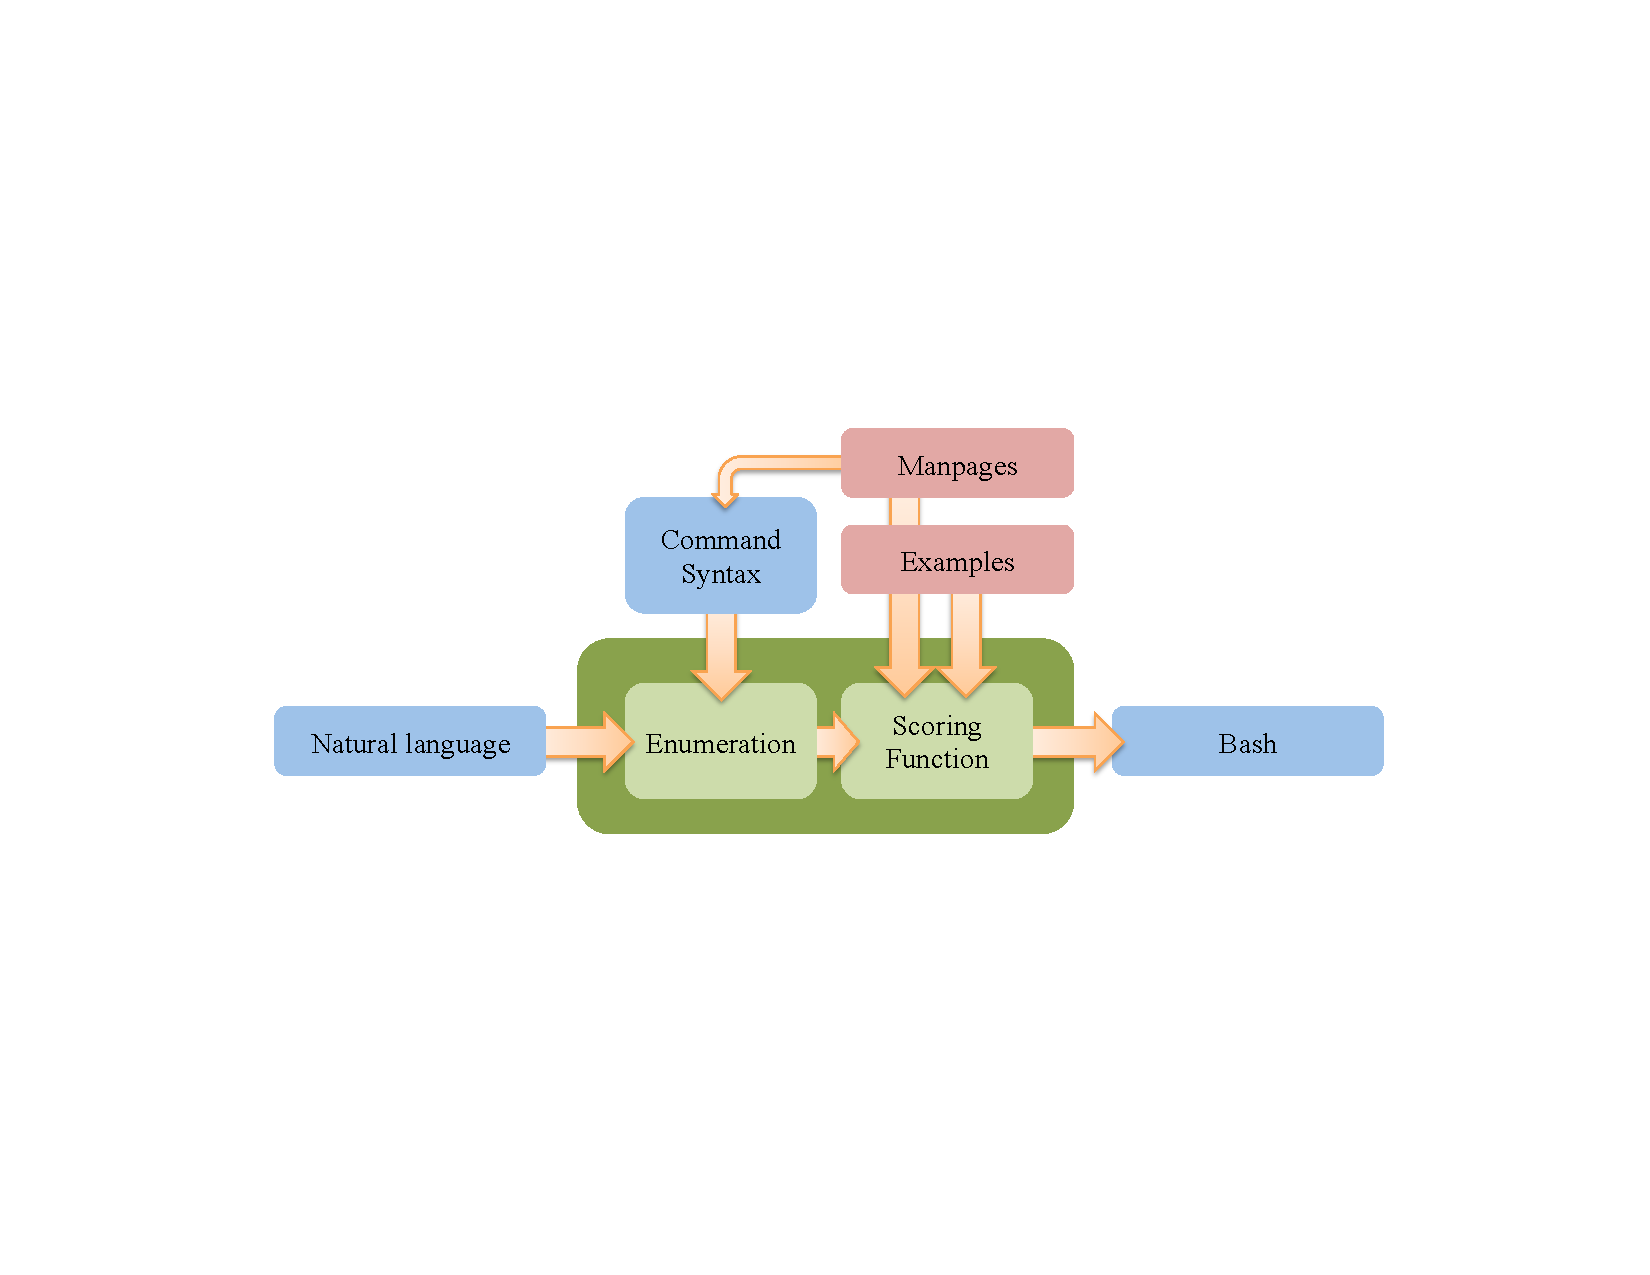
\includegraphics[width=4in]{architecture.pdf} \end{center}
    \caption{The overall architecture of our tool. Offline, the tool learns the
        valid syntax for common Bash commands using manpages. Both the manpages
        and a set of input-output examples are used to learn an appropriate
        scoring function. At runtime, the tool enumerates possible candidate
        programs using the learned syntax, scores them using the learned scoring
        function, and presents the top-ranked suggestions to the user.}
    \label{fig:arch}
\end{figure}

The natural language based command line interpreter we plan to develop consists of three key components: 1) an intermediate language  based on which Linux commands are generated and
% 2) a learning algorithm that can learn primitive commands of the intermediate language with provided man pages and 
2) a semantic parser that effectively maps the natural language commands issued by users to this intermediate representation. Especially, our initial pilot system is restricted to cover only file system operations, including file lookup, directory tree transformation, file content transformation, file property modifications. We restrict the domain in the hope that it can be expressed with tractable logic as well as to reduce the degree of ambiguity in the natural language command. Section~\ref{subsec:represent} introduces the formal language design and section~\ref{subsec:parser} introduces the approach to train the semantic parser.

\subsection{Language Design}
\label{subsec:represent}
An ideal intermediate language for the CLI programs should be 1) expressive enough so that it covers many interesting real world cases, 2) concise enough for the synthesizer to efficiently synthesize and 3) extensible, so that different people targeting different command line applications and use different sets of primitive commands.

Concretely, the syntax of the intermediate language design is presented below.

\begin{figure}
\[
\begin{array}{rlll}
\multicolumn{3}{l}{\textbf{Program}}\\
\mathit{p} & := & \mathit{value} \\
    &  & \mathit{cmd}~\overline{\mathit{flag}}~\overline{\mathit{arg}} & \textrm{(Program)}\\
    &  & \mathit{p} ~\| ~\mathit{p} & \textrm{(Pipelined program)}\\
\mathit{value} & := & \mathsf{date} ~|~ \mathsf{filename} ~|~ ... & \textrm{(Primitive values)}\\
\mathit{arg} & := & \epsilon ~|~ \mathit{value} ~|~ \mathit{hole} & \textrm{(Arguments)}\\
\mathit{cmd}^{*} & := & \mathsf{find} ~|~ \mathsf{grep} ~|~ ... & \textrm{(Commands)}\\
\mathit{flag}^{*} & := & \epsilon ~|~ -f ~|~ -h ~|~ ... & \textrm{(Flags)}\\
~\\
\multicolumn{3}{l}{\textbf{Command Signature}}\\
\mathit{sig} & := & \mathsf{name}~\mathit{option}:\tau & \textrm{(Command signature)}\\
\mathit{option} &:= & \mathsf{flagname} & \textrm{(Command option)}\\
                &   & \mathsf{argname}[\tau]\\
                &   & \mathit{option}~\mathbf{or}~\mathit{option}\\
                &   & [ \mathit{option} ]\\
~\\
\multicolumn{3}{l}{\textbf{Rules}}\\
\mathit{rule}^{*} &:=& \mathsf{find}~f[\mathsf{File}] : \mathsf{File}\\
                  &  & \mathit{date}~\mathit{-d} : \mathsf{void}\\
                  &  & \mathit{date}~\mathit{-u} : \mathsf{Date}\\
                  &  & ...\\
~\\
\multicolumn{3}{l}{\textbf{Types}}\\
\tau_0 & := & \mathsf{void} ~|~ \mathsf{File} & \textrm{(Primitive types)}\\
       &     & |~ \mathsf{Date} ~|~ \mathsf{Permission} ~|~ \mathsf{Size} ~|~ ... \\
\tau & := & \tau_0 ~|~ \tau_0\rightarrow \tau_0 & \textrm{(Type)}
\end{array}
\]
\caption{Intermediate Language}
\label{fig:lang}
\end{figure}


The first part of our language is the program syntax (labeled as \textbf{Program}), defines how a program can be formed: a CLI program can be 1) refer to a value, 2) call a primitive command, and 3) pipelining two programs and passing the result of the first program as the argument of the second program.

The rest of the language are designed to help check well-formedness of a given CLI program. The command signature defines how a rule can be written, the rules (\textbf{Rule}) defines which primitive programs are valid. Then, with the help of the types in our program, we can check the type of a program $p$ to ensure that a command line program is well-formed.

Since the number of basic Linux commands and options is large even in domain-specific scenarios, it is difficult for a human designer to hand-code all of the generation rules. We plan to semi-automate this step by adding information extracted from the Linux man pages\footnote{\url{http://linux.die.net/man/}} and make the language extensible. Concretely, we shall parse the man page to generate primitive commands, flags and checking rules for each command (all non-terminals labeled with * in Figure~\ref{fig:lang} will be automatically learned from man page). And with this language design, users can extend the basic language by providing man pages.

\subsection{Natural Language Command Interpreter}
\label{subsec:parser}
We train the natural language command interpreter using the Linux man pages, in addition to a small set of natural language and command line program pairs. The motivation of adopting man pages as one resource of the training data lies in the fact that gathering sufficient number of of natural language to command line program pairs is expensive. The large volume of Stack Overflow conversations are noisy and only a handful of high-quality training pairs can be confidently extracted. On the other hand, the Linux man pages are well formatted and contains rich natural language text that explains the usage of each command template and its possible arguments. We propose to use the command-explanation pairs extracted from man pages as additional signals to guide the search for high score rankings, thereby remedies the lack of example training pairs.

We use a linear feature function to score the natural language command to logical representation mappings. The following features are used:
\begin{itemize}\itemsep-1pt
	\item association of key words/phrases to partial expressions
	\item association between partial expressions (e.g. how often do they combined in valid commands)
	\item similarity of key words/phrases in the command to the man page explanation text of a partial expression
	\item complexity of the logical formulas and the commands generated from them.
\end{itemize}
We use the structured perceptron algorithm to learn weights of the scoring function from the example pairs. In each training iteration, we search for the top ranked logical form and update the weights based on its similarity to the ground truth logical form.
% We planned to extend learning into an interactive setting once the basic framework is developed.
%!TEX root=writeup.tex
\section{Experimental Evaluation}

Our key research question is:
%
\begin{quote}
    Can the tool described thus far improve the speed with which programmers
    accomplish tasks with the command line?
\end{quote}

\subsection{Methodology}

To answer this question we plan to conduct a small pilot user study. Programmers
will be asked to accomplish various tasks at the command line. They will be
divided into two groups: one group will be allowed to use our tool, and the
other will be allowed to use the internet. Both groups will be allowed the use
of manpages and will be allowed to experiment by running their commands.

We hypothesize that our tool will improve the speed with which programmers
devise solutions without impeding the correctness of those solutions.

\paragraph{Task} The programmers will each be asked to perform a small number of
tasks using the command line. The tasks will be drawn from our collected data.
Importantly, these tasks will be set aside before training the tool; they will
be novel examples.
A straightforward one-line solution exists for each task, although that solution
may use exotic commands or flags. The programmers will be allowed to produce
multi-line scripts as solutions, provided that those scripts correctly
automate the task. Some example tasks are listed in \autoref{fig:sample-tasks}.
We will not impose any specific time limit on the participants.

\begin{figure}[ht]
    \begin{framed}
    \begin{itemize}\itemsep-1pt
        \item In the current directory, recursively find all files with ``conf''
            in the filename
        \item Recursively remove all empty sub-directories from a directory tree
        \item Find files that are not executable
        \item Find the 100 biggest files on your system
        \item Make a tar archive of a folder, excluding .png files
    \end{itemize}
    \end{framed}
    \caption{Sample tasks for the proposed user study.}
    \vspace{-10pt}
    \label{fig:sample-tasks}
\end{figure}

\paragraph{Participants} The participants in the study will be undergraduate and
graduate students. They will be proficient command-line users, but not
necessarily experts. We expect to perform the study with at least five
participants in each group.

\paragraph{Measurements} We will primarily measure two things:
\begin{enumerate}\itemsep-1pt
    \item How long do participants take to perform each task?
    \item Are the participants' solutions correct?
\end{enumerate}
We will measure the participants' speed by having them specifically indicate
when they have completed each task. We will measure correctness by having them
save the output from each task; we will compare that output against the correct
solution.

\paragraph{Internal Measures} Additionally, we plan to quantify several internal
measures about the tool:
\begin{enumerate}\itemsep-1pt
    \item Performance: how long does training take to produce a model? How
        long does the tool take to answer a query?
    \item For a large number of hand-picked inputs, how often does the
        tool produce a correct answer?
    \item How often is the output close to correct, requiring only small
        adjustment? (``Small adjustment'' is defined as removing flags or
        changing arguments. Adding an argument, changing a command, or
        adding a pipe operator are not small adjustments.)
\end{enumerate}

\subsection{Results}

\todo{No results yet!}

%!TEX root=writeup.tex
\section{Discussion and Future Work}

Automatically generating bash commands based on natural language descriptions is a non-trivial AI task that fuses both natural language processing and program synthesis techniques. Based on the current result, we identify the following problems in our approach that lead to unsatisfactory result, and plans to fix these problems are listed along with the problems below.

\subsection{Dataset}

Using only noisy StackOverflow data as training data can lead to less satisfactory trained model due to the fact that the data size is still not big enough and the data quality are relatively low. Concretely, small data size results in the coverage issue: some command usage patterns are not covered in the dataset and the trained model cannot identify text describing these patterns. The low quality issue (containing mismatches between commands and texts) make the model learned some wrong translation patterns and thus damages translation quality. 

Based on this observation, we are planning to 1) enrich the current training data set with more (possibly noisy) examples to enhance the coverage of bash command usage and 2) collect a small but high quality data used as a separate training data source. The data sources we plan to obtain are listed below.
\begin{itemize}\itemsep-1pt
\item \textit{SuperUser forum.} SuperUser contains similar data as StackOverflow, but more specialized for system users, and thus can be used as complementary data to enrich the training data set.
\item \textit{Examples from Linux man page.} Besides defining the grammar of a command and explaining its usage, a Linux man page for a command also contain a section providing examples to demonstrate the usage of the command. Though small in the number, these examples are high quality training data that can be utilized, and they can be obtained by parsing the man pages.
\item \textit{Tutorial Examples.} Online bash command tutorials\footnote{http://ryanstutorials.net/linuxtutorial/filemanipulation.php}\footnote{http://www.ee.surrey.ac.uk/Teaching/Unix/} often contain a small set of clean explanation/command pairs. Due to the difficulty of automatically parsing different websites, we are planning to manually extract them from websites to create a data set containing  $\sim$300 examples.
\item \textit{Collecting data form colleagues.} One possibility of obtaining high quality data is to collect from colleagues who are familiar with bash commands. A ``command line programming challenge'' can be hosted to attract experts to write bash commands for our pre-selected natural language descriptions to obtain these data. We consider this method a backup that we are not planning to use in short-term future, but if other data sources are still not satisfactory, we shall come to this method. 
\end{itemize}

\subsection{Training Features}
\label{future:features}

In our current state of model training, only text-term co-occurrence feature is used and this limits the potential of the model. The following other features are planned to be added in training.
\begin{itemize}\itemsep-1pt
\item \textit{Naturalness.} Naturalness is of a command is measured by the co-occurrences of terms in a command. The inspiration of using this feature is that some generated commands contains unnatural term combinations. For example, a command \code{grep -i -l -o -w} is generated by the current approach with the input text ``Find all files from that contain word eth0.'', however, in this case, since the combination of \code{-l} and \code{-i} is not common in writing commands with \code{grep}. And the target of evaluating the naturalness is to help prevent a generated command with abnormal patterns.
\item \textit{TF-IDF scoring with man page.} Man pages provide explanations of all the options (flags, arguments) that can appear in a command. Thus, given texts describing what the desired command should looks like, comparing the similarity of user's text with the man page explanation can help locate what are the options may need to be used in the command. One natural way to compute the similarity is to first compute the TF-IDF score of the words in man pages, and them look up whether words in the user's text are top ranking words in a (option, explanation) pair, if it is, ``option'' is likely to be used in the generated command.  
\end{itemize} 

\subsection{Modeling Values}
\label{future:semantics}

In the current translation system, arguments in an generated command are not values extracted from the text but a dummy value with its type and users need to manually fill these dummy values. Based on our observation on text/command pairs in the data set, values in a command can come from the following sources: 1) a numeric or ordinal value in the text, e.g. a number `100' or a string `foo.txt' , 2) an implicit value requiring domain knowledge, e.g. current directory ``.'', root folder ``$\sim$''.

To enable a program to instantiate arguments during translation, the following processes are supposed to be added. 
\begin{itemize}\itemsep-1pt
\item Training a model to extract noun phrases in a command that represent values, which can be trained from the same data that is used to train the translation process.
\item Encoding domain knowledge about values as a dictionary that maps concepts into concrete values. E.g. file name, file date, file size, folder, subfolder, hidden file, executable file etc.
\end{itemize}

In some cases, the description text provided by the user may be ambiguous or unclear so that values cannot be directly learned from it. For example, an user asking the question ``how to copy the log file to another directory'' does not contains the information about what the concrete file or folder are. Thus, an interactive phase can be added to ask user to disambiguate the value in the question. For example, in this case, when the probability of ``the log file'' to be the actual value is low, we shall ask the user a question ``What does `the log file' in the question stands for?'', and the user may answer ``xxx.log'' so that the actual value to patch in the command can be obtained.


\bibliographystyle{abbrv}
\bibliography{bibliography}

\clearpage
\appendix
%!TEX root=writeup.tex
\section{Proposed User Study}
\label{sec:userstudy}

Our key research question is:
%
\begin{quote}
    Can the tool described thus far improve the speed with which programmers
    accomplish tasks with the command line?
\end{quote}
%
To answer this question we plan to conduct a small pilot user study. Programmers
will be asked to accomplish various tasks at the command line. They will be
divided into two groups: one group will be allowed to use our tool, and the
other will be allowed to use the internet. Both groups will be allowed the use
of manpages and will be allowed to experiment by running their commands.

We hypothesize that our tool will improve the speed with which programmers
devise solutions without impeding the correctness of those solutions.

\paragraph{Task} The programmers will each be asked to perform a small number of
tasks using the command line. The tasks are shown in \autoref{fig:tasks} and
will be drawn from our collected data. Importantly, these tasks will be set
aside before training the tool; they will not be examples the tool has seen
before.

There are several confounding factors to account for: some tasks may be easier
than others, some participants may be more experienced than others, and the
tasks may become easier for the participants as they progres. To control for
these, the tasks have been randomly split into two blocks $T_1$ and $T_2$.
Each participant will each block under one of two setups:
\begin{itemize}
    \item $S_1$ --- access to local manpages and the internet
    \item $S_2$ --- access to local manpages and our tool
\end{itemize}

There are four possible combinations of (block, setup) assignments and
orderings; participants will be randomly assigned to one of these four groups:
\begin{itemize}
    \item $T_1 S_1$, $T_2 S_2$ --- task 1 under setup 1 followed by task 2 under setup 2
    \item $T_1 S_2$, $T_2 S_1$ --- task 1 under setup 2 followed by task 2 under setup 1
    \item $T_2 S_1$, $T_1 S_2$ --- task 2 under setup 1 followed by task 1 under setup 2
    \item $T_2 S_2$, $T_1 S_1$ --- task 2 under setup 2 followed by task 1 under setup 1
\end{itemize}

While the tasks all have one-line solutions, those solutions may involve exotic
commands or flags. The programmers will be allowed to produce multi-line scripts
as solutions, provided that those scripts correctly automate the task. We will
not impose any specific time limit on the participants.

\begin{figure}[ht]
    \begin{subfigure}[b]{0.48\textwidth}
        \begin{framed}
        \begin{itemize}\itemsep-1pt
            \item In the current directory, recursively find all files with ``conf''
                in the filename
            \item Recursively remove all empty sub-directories from a directory tree
            \item Find files that are not executable
            \item Find the 100 biggest files on your system
            \item Make a tar archive of a folder, excluding .png files
        \end{itemize}
        \end{framed}
        \caption{Task set $T_1$}
    \end{subfigure}
    \begin{subfigure}[b]{0.48\textwidth}
        \begin{framed}
        \begin{itemize}\itemsep-1pt
            \item ...
            \item ...
            \item ...
            \item ...
            \item ...
        \end{itemize}
        \end{framed}
        \caption{Task set $T_2$}
    \end{subfigure}
    \caption{Tasks for the user study, randomly divided into two groups.}
    \vspace{-10pt}
    \label{fig:tasks}
\end{figure}

\paragraph{Participants} The participants in the study will be undergraduate and
graduate students. They will be proficient command-line users, but not
necessarily experts. We expect to perform the study with at least five
participants in each group.

\paragraph{Measurements} We will primarily measure two things:
\begin{enumerate}\itemsep-1pt
    \item How long do participants take to perform each task?
    \item Are the participants' solutions correct?
\end{enumerate}
We will measure the participants' speed by having them specifically indicate
when they have completed each task. We will measure correctness by having them
save the output from each task; we will compare that output against the correct
solution. \autoref{tbl:user-study-results} shows a placeholder table for what
numbers we would be interested in reporting.

\begin{table}
    \begin{center}
    \begin{tabular}{lrr}
        \textbf{Task/Setup} & \textbf{Without (s)} & \textbf{With (s)} \\
        \hline
        $T_1 S_1$, $T_2 S_2$ & - & - \\
        $T_1 S_2$, $T_2 S_1$ & - & - \\
        $T_2 S_1$, $T_1 S_2$ & - & - \\
        $T_2 S_2$, $T_1 S_1$ & - & - \\
    \end{tabular}
    \end{center}
    \caption{User study results. The ``Task/Setup'' column shows that tasks
        would be performed under what setups and in what order. The ``Without (s)''
        column shows the average time taken by participants on the task with
        setup 1 (manpages+internet). The ``With (s)'' column shows the average
        time taken by participants on the task with setup 2 (manpages+tool).}
    \label{tbl:user-study-results}
\end{table}

\paragraph{Internal Measures} Additionally, we plan to quantify several internal
measures about the tool:
\begin{enumerate}\itemsep-1pt
    \item Performance: how long does training take to produce a model? How
        long does the tool take to answer a query?
    \item For a large number of hand-picked inputs, how often does the
        tool produce a correct answer?
    \item How often is the output close to correct, requiring only small
        adjustment? (``Small adjustment'' is defined as removing flags or
        changing arguments. Adding an argument, changing a command, or
        adding a pipe operator are not small adjustments.)
\end{enumerate}


\end{document}
